\documentclass[english]{report}

\usepackage[left=1in, right=1.0in, top=1.0in, bottom=1.0in]{geometry}
\usepackage{layout}
\usepackage{amsmath}
\usepackage{graphicx}
\usepackage{babel}

% R code colorization
% based on http://stackoverflow.com/questions/21402157/colour-for-r-code-chunk-in-listings-package/21468454#21468454
\usepackage{listings}             % Include the listings-package
\usepackage[usenames,dvipsnames]{color}    
 \lstset{ 
  language=R,                     % the language of the code
  basicstyle=\ttfamily, % the size of the fonts that are used for the code
  numbers=left,                   % where to put the line-numbers
  numberstyle=\tiny\color{Blue},  % the style that is used for the line-numbers
  stepnumber=1,                   % the step between two line-numbers. If it's 1, each line
                                  % will be numbered
  numbersep=5pt,                  % how far the line-numbers are from the code
  backgroundcolor=\color{white},  % choose the background color. You must add \usepackage{color}
  showspaces=false,               % show spaces adding particular underscores
  showstringspaces=false,         % underline spaces within strings
  showtabs=false,                 % show tabs within strings adding particular underscores
  frame=single,                   % adds a frame around the code
  rulecolor=\color{black},        % if not set, the frame-color may be changed on line-breaks within not-black text (e.g. commens (green here))
  tabsize=2,                      % sets default tabsize to 2 spaces
  captionpos=b,                   % sets the caption-position to bottom
  breaklines=true,                % sets automatic line breaking
  breakatwhitespace=false,        % sets if automatic breaks should only happen at whitespace
  keywordstyle=\color{RoyalBlue},      % keyword style
  commentstyle=\color{YellowGreen},   % comment style
  stringstyle=\color{ForestGreen}      % string literal style
} 

\begin{document}

\begin{titlepage}
\begin{center}

% Upper part of the page. The '~' is needed because \\
% only works if a paragraph has started.
%\includegraphics[width=0.15\textwidth]{./logo}~\\[1cm]

\textsc{\LARGE University of Waterloo}\\[1.5cm]

\textsc{\Large Stat440 Project}\\[0.5cm]

% Title
%\HRule \\[0.4cm]
{ \huge \bfseries The Normal|Inverse-Wishart Sampler \\[0.4cm] }

%\HRule \\[1.5cm]

% Author and supervisor
\begin{minipage}{0.4\textwidth}
\begin{flushleft} \large
\emph{Authors:}\\
Daniel \textsc{Galperin} 20351954\\
Nick \textsc{Guenther} 20230268
\end{flushleft}
\end{minipage}
\begin{minipage}{0.4\textwidth}
\begin{flushright} \large
\emph{Supervisor:} \\
~Martin \textsc{Lysy}
\end{flushright}
\end{minipage}

%\vfill

\end{center}
\end{titlepage}

% 1 page
%\maketitle


% this should be 10 pages: 1 page title, 1 page references, 8 pages of content

%\layout %debugging print for margins


\newpage

\tableofcontents %because latex is from before the days of interactive computing, you need to run the build twice for this to show up
 % also note that only autonumbered sections get entered into the TOC by default
 % see http://www.andy-roberts.net/writing/latex/contents

%these macros correct part of the oversight:
% of couse, these macros also confuse texmaker
% le sigh
\newcommand{\Section}[1] {
  \section*{#1}
  \addcontentsline{toc}{section}{#1}
}

\newcommand{\Subsection}[1] {
  \subsection*{#1}
  \addcontentsline{toc}{subsection}{#1}
}

\newcommand{\Subsubsection}[1] {
  \subsubsection*{#1}
  \addcontentsline{toc}{subsubsection}{#1}
}

% .5 pages
\Section{Introduction}
% some of section below from wikipedia
The Normal-Inverse Wishart distribution is a multivariate four-parameter family of continous probability distributions.
%.....

%its history
%its relationship to other others (it's a generalized Normal-Inverse-ChiSq)

%In bayesian statistics, it is the conjugate prior in (...this situation...)

Its main use is as the conjugate prior for a multivariate normal distribution with unknown mean and covariance matrix.

%Due to its common use in bayesian statistics, Generating samples from this distribution is often the bottleneck in generating the %credible interval. 

The main goal of this package is to provide functions written in Rcpp\cite{Rcpp} to help with Bayesian analysis related to the Normal Inverse-Wishart distribution.

While there are libraries that can generate Inverse-Wishart samples, such as MCMCpack\cite{MCMCpack} and LaplaceDemon\cite{LaplaceDemon}, there is currently no library that directly samples Normal-Inverse-Wisharts. While it is possible to use those to construct NIW samples from those, it requires extra effort on the user and is likely to be less effient than our method as generating Normals would be done in R.

Our package also provides MNIW samples, which no package currently provides, as well as a function to generate samples for B and V in multilinear regression(see examples).
% (4 pages)
\Section{Program Package}

% 1 page
\Subsection{Algorithm}

- Why we care
- State of the art
  - MCMCpack
  ```
  > riwish
  function (v, S) 
  {
      return(solve(rwish(v, solve(S))))
      }
   ```   
 there's also rinvwishartc and dinvwishartc in LaplacesDemon(http://www.bayesian-inference.com/softwaredownload) 
   AND there's a version which is cholesky-parameterized
  but their version strictly only does one random matrix at a time
  
- What we did differently
  tuse this cholesky trick ... 

% (2?? pages)
\Subsection{Testing}

% 1 pages
\Subsubsection{Correctness <-- this title is dumb}

There is no test we can do which will demonstrate the correctness of this code.
Like Knuth, we have only proven this code correct, not tested it thoroughly.
But there are some relatively basic tests we have applied to 
(- brief mention that doing a full multivariate K-S test is so hard as to be ridiculous (+ citation?))

Each element we are generating has a distribution by itself. These are the \emph{marginal distributions} such as:

$$ V_{2,3} | X_1, X_2, X_3, ..., V_{1,1}, V_{1,2}, V_{1,3} , ....  \sim P(V_{2,3} = v) $$
% BUG: continuous distributions don't have "equals"
%  I wish there was a consistent notation which covered the discrete and continuous cases together without having to jump a layer of indirection into pdfs

We can derive the marginals directly. For the elements of $X$, we have:


so  $X_i \sim t_{???}$ .

For the elements of $V$, we have:

....


More quickly, we can sample $X,V \sim NIW$ from a sampler that we know should work: the naive algorithm %TODO: <-- grammar%
  , and then use kernel density estimation.
  
With either method, we get a PDF, and we can plot histograms and the PDF together. Here are some examples of this from our final code:

(IMAGE: A correct sample)
(IMAGE: An incorrect sample)


Every \emph{moment} is an expected value. This makes moments an easy to compute statistic,
 because (for $ S_i \sim S $)
$$ lim_{n \rightarrow \infty} \frac{\sum_{i=1}^n g(S_i)}{n} = E[g(S)] $$
  ((TODO: prove. why is this? the CLT??))
so we can just take samples, map them with a function, and average. As more samples come in we expect these numbers to converge to specific values. As before, we can examine the marginals one by one. We can check for convergence by.

Our moments are multivariate, so as before we need to look at marginals 
(IMAGE: an element moment converging to the expected value)

Finally, we used a k-s test [CITE?] to numerically detect marginals which deviate from the correct value. Example 
```
snappy2 X[3]: different
snappy2 X[4]: same
snappy2 V[1,1]: same
snappy2 V[1,2]: same
snappy2 V[1,3]: different
```


If, under a large number of samples, any of these statistics ((is it correct to call a full pdf a 'statistic'? you could view a function as an infinite set related statistics...)) do not match its expected value--pdf or moment--it means there is an error. Conversely, while all of the statistics matching doesn't logically prove correctness, they give strong support to likelihood of correctness.



% 1 page
\Subsubsection{Benchmarking}


We implemented several versions of the NIW sampler. We tested its runtime by varying $n$, the number of samples. We did not test varying $d$, the dimensionality of the output. Sketches of each implementation are in the appendix. Figure 1 shows the runtimes of each implementation.

\begin{figure}[hbtp]
\centering
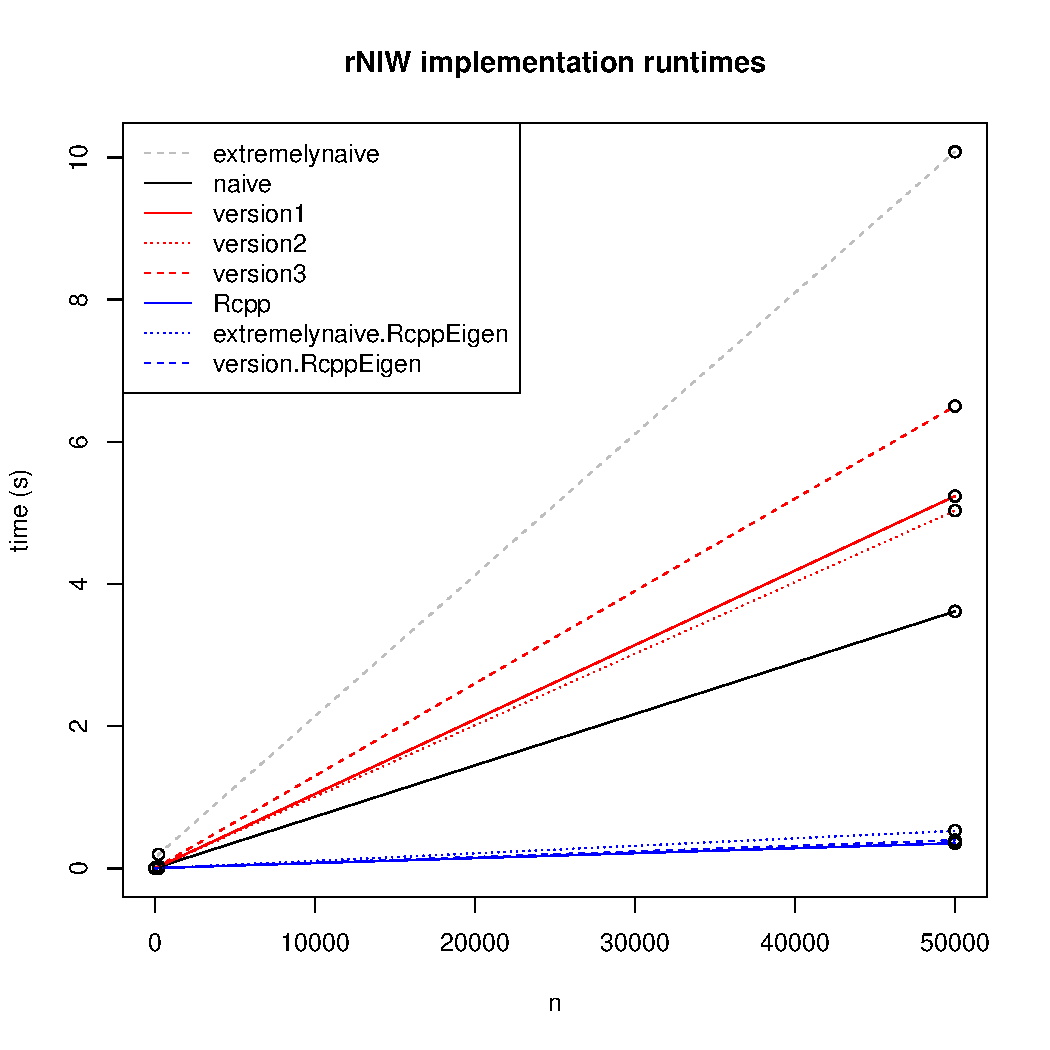
\includegraphics[scale=.5]{runtimes.pdf}
\caption{Implementation runtimes. The naive algorithms are monochrome; the efficient algorithm prototyped in R is red; the C implementations (naive and efficient) are blue.}
\end{figure}

As expected, the runtime is linear in $n$, since every sample of the $n$ is generated identically. We fit lines to each algorithm's runtime to estimate their scaling coefficient. We picked \emph{naive} as a baseline and put all algorithm frequencies on a relative scale.

\begin{table}[ht]
\caption{\emph{rNIW} Runtimes}
\begin{center}
\begin{tabular}{rrrr}
    algorithm       & slope  &      ratio   &        sd\\
    \hline
              \emph{extremelynaive}   &4918.468  & 0.35 & 3.43e-05 \\
                \emph{version3}   &7648.601 & 0.55 & 1.82e-06 \\
               \emph{version1}   &9543.389 & 0.69 &2.57e-04 \\
                \emph{version2}   & 9980.602 & 0.72 & 1.54e-04 \\
                   \emph{naive}  &13890.529  & 1.00 & 7.27e-04 \\
  \emph{extremelynaive.RcppEigen} & 94128.482 & 6.78 & 3.96e-03 \\
        \emph{version.RcppEigen} & 125032.317  & 9.00 & 4.38e-03 \\
                     \emph{Rcpp} & 143356.322  & 10.32 & 3.97e-02 \\
    \hline
\end{tabular}
\caption{Runtime summary:     
    \emph{slope} is each algorithm's performance samples/second, \emph{ratio} is the ratio of each against "naive"; \emph{sd} is the standard deviation of \emph{ratio}. Sorted in order or performance, worst to best.}
\end{center}
\label{tab:multicol}
\end{table}


These results show that our algorithm gets about a 25 times times speed up over the extremely naive algorithm. But this is misleading: the naive algorithm that an R user would reach for would is not the deeply naive algorithm, but rather what we wrote as \emph{naive}, where we call out to R's built in \emph{rWishart} function. Compared to this version, our blazing fast best implementation is only 10 times better. The explanation is that almost all of the naive algorithm's output, the $n \cdot d^d$ entries of $V$, are constructed at the C level, because \emph{rWishart} is a native function. The sheer amount of time that this saves makes the naive algorithm faster than all of our R implementations of the efficient algorithm.

There is another unusual result: the algorithm written with more \emph{backsolve}s (\emph{version3}) is slower than the one without, even though \emph{backsolve} is a $O(d^2)$ algorithm and matrix multiply is $O(d^3)$ \cite{?????}. This might be an artifact of our only testing on small matrices, where a direct multiply is better, though.

% (4 pages?)
\Section{Application}

The NIW distribution is a extremely common conjugate prior. Here, we use our algorithm to rapidly do a simulation study:

% 1.25 pages
\Subsection{Multi-variable Regression}

One use of the NIW distribution is to get distributions and credible intervals for parameters and variance in multivariable regression.\\

Let $X_{n\times p} = [x_{ij}]$ and $Y_{n\times q} = [y_{ij}]$ be matrices of p predictors and q respones for each of n observations, and let $E_{n\times q}$ be the matrix of errors. The regression model is

\[Y = X\beta + E, (\epsilon_{i1},\hdots,\epsilon_{i q})\sim N_q(0,V)\]

where $\beta_{p\times q} = [\beta_{ij}] $ and $V_{q\times q}$. The conjugate prior for the model is:

\begin{align*}
	V &\sim  Inv-W_q(\Psi,\nu)\\
	\beta|V &\sim N_{pq}\{\Lambda, V  \otimes \Omega^{-1}\}
\end{align*}

The parameters of the prior are $\Psi_{q\times q}, \nu_{1\times 1}, \Lambda_{p\times q}, \Omega_{p\times p}$\\

The resulting posterior distribution is.


\begin{align*}
	V|Y,X &\sim  Inv\text{-}W_q(\Psi+S+C,\nu+n)\\
	\beta|V,Y,X &\sim N_{pq}\{A\Lambda + (I-A)\hat{\beta}, V  \otimes (X'X +\Omega)^{-1}\}
\end{align*}
where 
\begin{align*}
\hat{\beta} &= (X'X)^{-1}X'Y\\
S &= (Y-X\hat{\beta})(Y-X\hat{\beta})\\ 
A &= (X'X + \Omega)^{-1}\Omega\\
C &= \hat{\beta}'(X'X)\hat{\beta} + \Lambda'\Omega\Lambda - (X'X\hat{\beta} + \Omega\Lambda)'(X'X+\Omega)^{-1}(X'X\hat{\beta} + \Omega\Lambda)
\end{align*}


lm.multivariable(...) is the function that generates B and V given X, Y, and the priors. The code for it is in the appendix, and next section shows a usage example.


\Subsubsection{Boston housing data example}

Using data from Boston in MASS, we tried to find the coefficients if trying to predict 6 of the parameters based on the other 8. as well as determine credible intervals for B and V\\
The code below demonstrates the process, as well as how you can use the result

\begin{lstlisting}[frame=single, language=R]
require(MASS)
D <- Boston
Y <- D[c("crim", "zn", "indus", "tax", "black", "lstat")]
X <- D[c("chas", "nox", "rm", "age", "dis", "rad", "ptratio", "medv")]

# One example using flat priors and df of 73

Result <- lm.multivariable(100000,as.matrix(X),as.matrix(Y))

# Now that we have that, we can generate 95% credibility interval
#by generating lower and upper quantiles

apply(Result$B, c(1,2), quantile, probs = 0.025)
#        [,1]       [,2]        [,3]        [,4]       [,5]        [,6]
#[1,] -2.4726166 -5.8679744  0.09608906 -32.9824267 -11.281075 -1.55826198
#[2,] -6.9573162 -0.8674746 20.12296722 256.4240012  71.771290 12.86687197
#[3,]  0.6781378  1.6702512 -1.27047227  -2.1000956 -14.681060 -1.33368492
#[4,] -0.1553847 -0.4728362 -0.09345642  -1.6003269  -1.790386 -0.08581789
#[5,] -0.5264732  6.4092475 -0.97953076   0.1691556   8.454171  0.20377180
#[6,]  0.4767344  0.2930137  0.04739809  13.7503723  -5.358764 -0.03775675
#[7,] -0.1783143 -2.4605295  0.36683531   4.8444292  11.568813  0.34594612
#[8,] -0.2359186  0.1865307 -0.06683020  -1.3784741   3.828851 -0.31275303

apply(Result$B, c(1,2), quantile, probs = 0.975)
apply(Result$V, c(1,2), quantile, probs = 0.025)
apply(Result$V, c(1,2), quantile, probs = 0.975)

# Example with non-flat priors

q <- dim(Y)[2];
p <- dim(X)[2]

Psi <- diag(q);
df <- 100;
Lambda <- matrix(1, p,q);
Omega <- diag(p);

Result <- lm.multivariable(100000,as.matrix(X),as.matrix(Y), 
                    Psi = Psi, Lambda = Lambda, Omega = Omega, df  = df)
                    
apply(Result$B, c(1,2), quantile, probs = 0.025)
apply(Result$B, c(1,2), quantile, probs = 0.975)
apply(Result$V, c(1,2), quantile, probs = 0.025)
apply(Result$V, c(1,2), quantile, probs = 0.975)


# Can also take a histogram to take a look a the distribution
# one example:

hist(Result$B[1,1,], breaks = 100, probability = TRUE)

\end{lstlisting}
% 1.25 pages
%\Subsection{Gibbs Sampler}

%- we did this thing
%- here's our test case
%- and look, the code is reusable (and in C)

% .5 pages
\Section{Conclusion}

We implemented a Matrix-Normal-Inverse-Wishart sampler and proved its use. It is definitely an improvement over what an R user would use before, but it is not as strikingly better as one might hope in 
In this report, we have demonstrated the accuracy and speed of our implementation of the NIW sampler as well as provided examples on how it can be used. 

% Put stuff not yet done that we plan to do or wish we could do
Parallelization and GPUs 


We offer this code \cite{MNIW} up in the hope it will make large linear models with an inverse-wishart prior tractable to the working statistician.



% 1 page
\newpage


\begin{thebibliography}{9}

\bibitem{R}R Core Team (2014). R: A language and environment for statistical computing. R Foundation for
  Statistical Computing, Vienna, Austria. URL http://www.R-project.org/.
  
\bibitem{Rcpp} Dirk Eddelbuettel and Romain Francois (2011). Rcpp: Seamless R and C++ Integration. Journal of
  Statistical Software, 40(8), 1-18. URL http://www.jstatsoft.org/v40/i08/.

\bibitem{RcppEigen}Douglas Bates, Dirk Eddelbuettel (2013). Fast and Elegant Numerical Linear Algebra Using the
  RcppEigen Package. Journal of Statistical Software, 52(5), 1-24. URL
  http://www.jstatsoft.org/v52/i05/.
\bibitem{MCMCpack}Andrew D. Martin, Kevin M. Quinn, Jong Hee Park (2011). MCMCpack: Markov Chain Monte Carlo in R.
  Journal of Statistical Software. 42(9): 1-21. URL http://www.jstatsoft.org/v42/i09/. 
 
\bibitem{LaplaceDemon}Statisticat, LLC. (2014). LaplacesDemon: Complete Environment for
  Bayesian Inference. Bayesian-Inference.com. R package version
  14.04.05. [http://www.bayesian-inference.com/software] 
 
\bibitem{MNIW}Daniel Galperin and Nick Guenther. (2014). MNIW. Version pre-alpha. [http://www.github.com/kousu/MNIW]
 
 \end{thebibliography}


\newpage

\Section{Appendix}

\Subsection{rNIW Implementations}

For brevity, only the unique portions of each implementation are shown.

\Subsubsection{"Naive" implementations}

\begin{figure}
\begin{lstlisting}[frame=single, language=R]
  d = length(Mu)
  ans = rNIW.alloc(n,d)
  
  for(i in 1:n) {
     ans$V[,,i] = rInvWishart(1, df, Psi)[,,1];
     ans$X[,i] = rmvnorm(1, Mu, ans$V[,,i]/kappa);
  }
\end{lstlisting}
\caption{\emph{extremelynaive}}
\end{figure}


\begin{figure}
\begin{lstlisting}[frame=single, language=R]
  ans$X = matrix(NA, d, n)
  ans$V = rInvWishart(n, df, Psi);   
  
  # unfortunately, generating X must still be in a loop because each sample has a different distribution
  # and there's no way with rmvnorm to ask "give me n samples and here's the parameters for each"
  # ..is there?
  #
  for(i in 1:n) {
     ans$X[,i] = rmvnorm(1, Mu, ans$V[,,i]/kappa);
  }
\end{lstlisting}
\caption{\emph{naive}}
\end{figure}

\begin{figure}
\begin{lstlisting}[frame=single, language=C]
// [[Rcpp::export]]
List rNIW_extremelynaive_eigen(unsigned int n, NumericVector Mu, double kappa, NumericMatrix Psi, double df) {
  // precondition: all the preconditions have been properly checked by rNIW.typechecked
  unsigned int d = Mu.length();
  
  NumericVector V(Dimension(d,d,n));
  NumericVector X(Dimension(d,n));
  
  for(unsigned int i=0; i<n; i++) {
    NumericMatrix Vi = riwishart(Psi, df);

    for(int j=0; j<d; j++) {
    for(int k=0; k<d; k++) {
      V[d*d*i + j*d + k] = Vi(j, k); //XXX this might be the wrong order (but V is symmetric so we can't tell)
    }
    }

    // hack: Rcpp "helpfully" has a whole slew of pseudo-symbolic classes ("Times_Vector_Vector") that it spits out when you try to do operands
    //  I can't tell if you can actually make it collapse things down
    //  So i'm going to use Eigen as a workaround
    // changing the definition of Vi in the process
    Vi = Rcpp::wrap(as<Map<MatrixXd> >(Vi) / kappa);
    //Rcout << "Vi[1,2] = " << Vi[1,2] << std::endl; //DEBUG
    NumericVector Xi = rmvnorm(1, Mu, Vi);
    for(int j=0; j<d; j++) {
      X[d*i + j] = Xi(j);
    }
    
  }

  return List::create(Named("X") = X, Named("V") = V);
}
\end{lstlisting}
\caption{\emph{extremelynaive.RcppEigen}}
\end{figure}


\Subsubsection{"Efficient" implementations}

\begin{figure}
\begin{lstlisting}[frame=single, language=R]
BartlettFactor <- function(d, df) {
  A = matrix(nrow=d, ncol=d)
  A[,] = 0
  df = df-(1:d)+1
  diag(A) = sqrt(rchisq(d, df))
    
  # set the below-diagonals to N(0,1)s
  i_lower = col(A) > row(A)
  A[i_lower] = rnorm(sum(i_lower))
  
  A
}
\end{lstlisting}
\caption{\emph{BartlettFactor}, upon which the efficient algorithm is founded.}
\end{figure}


\begin{figure}
\begin{lstlisting}[frame=single, language=R]
  gamma.inv = solve(chol(solve(Psi)))
  for(i in 1:n) {    
    # construct the cholesky decomposition of a W(I, df) 
    A = BartlettFactor(d, df)
    
    A.inv = backsolve(A, I)
    U.inv = gamma.inv %*% A.inv
    
    ans$V[,,i] = tcrossprod(U.inv) #note well that this is not a LU decomposition -- it's UL
    
    # now we want X ~ N(Mu, V/kappa)
    z = rnorm(d); vector
    ans$X[,i] = Mu + U.inv %*% z/sqrt(kappa)
  }
\end{lstlisting}
\caption{\emph{version1}, the basic (should-be) efficient algorithm.}
\end{figure}


\begin{figure}
\begin{lstlisting}[frame=single, language=R]
  gamma.inv = solve(chol(solve(Psi)))
  for(i in 1:n) {
     
     A = BartlettFactor(d, df)
     A.inv = backsolve(A, I)
     
     z = rnorm(d);
     
     U.inv = gamma.inv %*% A.inv
     ans$V[,,i] = tcrossprod(U.inv)
     ans$X[,i] = U.inv %*% z
  }
  ans$X =  Mu + ans$X/sqrt(kappa) 
\end{lstlisting}
\caption{\emph{version2}, which uses R's vectorization syntax.}
\end{figure}

\begin{figure}
\begin{lstlisting}[frame=single, language=R]
  gamma = chol(solve(Psi))
  
  for(i in 1:n) {  #apply scaling after the fact
     
     A = BartlettFactor(d, df)
     
     U = A %*% gamma
     
     # sample V
     U.inv = backsolve(U, I) 
     ans$V[,,i] = tcrossprod(U.inv)
     
     # sample X
     z = rnorm(d);
     ans$X[,i] = backsolve(U, z)
  }
  ans$X =  Mu + ans$X/sqrt(kappa) 
\end{lstlisting}
\caption{\emph{version3}, which uses \emph{backsolve} instead of a normal matrix multiply.}
\end{figure}


\begin{figure}
\begin{lstlisting}[frame=single, language=R]
  # precompute some useful values
  d = length(Mu)
  gamma.inv = solve(chol(solve(Psi)))
    
  return(rNIW_Rcpp(n, d, Mu, kappa, gamma.inv, df))
\end{lstlisting}
\caption{\emph{Rcpp}, R side of the code}
\end{figure}

\begin{figure}
\begin{lstlisting}[frame=single, language=C]
 // [[Rcpp::export]]
SEXP rNIW_Rcpp(int n, int d, NumericVector Mu, double kappa, NumericVector gamma_inv, double df) {
  NumericVector V_ans(Dimension(d,d,n));
  NumericVector X_ans(Dimension(d,n));
  
  
  NumericVector A(Dimension(d,d));
  for (int k = 0; k < n; k++){
   // First, create A.
  BartlettFactorCpp(d,df, A);
    // Apply backsolve
  NumericVector A_inv = backSolveInverse(A,d);
  
  NumericVector z = rnorm(d);
  
  
  NumericVector U_inv(Dimension(d,d));
  // might want to move this to helper function for upper triangular dot product
  for (int col = 0; col < d; col++){ // col of result 
    for(int row = 0; row < d; row++){ // row of result
      for(int i = 0; i < d; i++){
        U_inv[col*d+row] +=  gamma_inv[i*d + row] * A_inv[col*d + i]; // Will optimize after
      }
               // Rcout << U_inv[col*d+row] << " ";
    }  
 //   Rcout << std::endl;
  }
  
  for (int col = 0; col < d; col++){
    for (int row = 0; row < d; row++){
      for(int i = 0; i < d; i++){
        V_ans[k*d*d + col*d + row] += U_inv[i*d + row] * U_inv[i*d + col];  
      }
    }
  }
  
  for(int i = 0; i < d; i++){
    for(int j = 0; j < d; j++){
      X_ans[k*d+i] += U_inv[j*d + i]*z[j];
    }
      X_ans[k*d + i] = X_ans[k*d + i]/sqrt(kappa) + Mu[i];
  }
  
  }
   List ret;
   ret["X"] = X_ans;
   ret["V"] = V_ans;
   return ret;
}
 
\end{lstlisting}
\caption{\emph{Rcpp}, C side of the code}
\end{figure}


\begin{figure}
\begin{lstlisting}[frame=single, language=C]
// [[Rcpp::export]]
List rNIW_version_eigen(unsigned int n, NumericVector Mu, double kappa, NumericVector Psi, double df) {
  // precondition: all the preconditions have been properly checked by rNIW.typechecked
  unsigned int d = Mu.length();

  NumericVector V(Dimension(d,d,n));
  NumericVector X(Dimension(d,n));

  // invert Psi  
  MatrixXd Psi_inv = as<Map<MatrixXd> >(Psi).inverse();
  // TODO: exploit that we know Psi is symmetric (but SelfAdjointView does not contain inverse()!! maybe knowing the matrix is symmetric doesn't help, in that case??)
  // factor Psi
  MatrixXd Gamma = Psi_inv.llt().matrixU();

  NumericVector A = NumericVector(Dimension(d,d));
  for(unsigned int i=0; i<n; i++) {
    // step 1: generate the bartlett factor..
    BartlettFactorCpp(d, df, A);
    MatrixXd A_ = as<Map<MatrixXd> >(A);  //map into Eigen so we can use linear algebras
    //TriangularView<MatrixXd, Upper> trA_ = A_.triangularView<Upper>();
    MatrixXd U = A_*Gamma;
    MatrixXd U_inv = U.inverse();
    MatrixXd Vi = tcrossprod(U_inv);
    // memcpy the result out of Eigen and into Rcpp
    // XXX does this need to be done manually? can't we call some "copy this block of memory" operation?
    for(int j=0; j<d; j++) {
    for(int k=0; k<d; k++) {
      V[d*d*i + j*d + k] = Vi(j, k); //XXX this might be the wrong order (but V is symmetric so we can't tell)
    }
    }
    
    // step 2: generate X
    VectorXd Xi = U.triangularView<Upper>().solve(as<Map<VectorXd> >(rnorm(d))); // backsolve(U, z)
    Xi /= sqrt(kappa);
    Xi += as<Map<VectorXd> >(Mu);
    for(int j=0; j<d; j++) {
      X[d*i + j] = Xi(j);
    }
    
  }  

  return List::create(Named("X") = X, Named("V") = V
       //extra debugging stuff
       //, Named("Psi.inv") = Psi_inv
       //, Named("Gamma") = Gamma
       );
}
\end{lstlisting}
\caption{\emph{version.RcppEigen}}
\end{figure}




\Subsection{Multivariable Regression}

\begin{lstlisting}[frame=single, language=R]
lm.multivariable <- function(m, X, Y, Lambda=NULL, Omega=NULL, Psi=NULL, df=71) { # TODO: Not sure what to name this.
  # Multivariable Regression via Bayesian Reasoning
  # 
  # This fits the model Y = XB + E where (E_i)^T ~iid MultiNormal(0, V)
  #  but it doesn't fit it in the frequentist sense of constructing
  #  true values for B and V -- instead it produces samples from the
  #  Bayesian Posterior.
  # The posterior, like a good little bayesian, is conjugate in this case:
  #  both the prior and the posterior are Matrix-Normal|Inverse-Wisharts.
  #
  # args:
  #  m: the number of samples to take
  #  X, Y: the observed data; these should be (n,q) and (n,d)
  #  Psi, df, Lambda, Omega: your prior knowledge, encoded
  #    as parameters of the Normal|Inverse-Wishart distribution.
  #   You should provide a df (though this won't make a huge difference)
  #    but, for convenience, by default the other parameters are set
  #    to give "flat" (aka uninformative aka improper) priors. 
  #   The flat prior on Omega causes Lambda to be ignored
  #    (hence its default value: NULL), and, as a special exception,
  #    causes the degrees of freedom of the posterior to change
  #     from (df+n) to (df+n-d).
  #  The flat prior on Psi is orthogonal to the flat prior on Omega (XXX is this true? surely it has some effect, even if only numerical/speed/something)
  #  (the argument order is chosen to reflect the distribution,
  #  which is the result of sampling
  #      MatrixNormal(Lambda, Omega, InverseWishart(Psi, df)), 
  #   though it does makes calling this function awkward)
  # 
  # returns:
  #  a list containing the posterior samples:
  #   $B
  #   $V
  
  n <- dim(X)[1];
  stopifnot(n == dim(Y)[1])
  q <- dim(Y)[2];
  d <- dim(X)[2];
  
  # TODO: can add some checks here
  
  #X'X is used often, only time X is used by itself is in S
  X.sq <- crossprod(X)
  
  # this posterior is neat:
  # it actually involves taking the usual frequentist fit (as produced by lm())
  #  B = (X'X)^{-1}X'y
  # and trading off between that fit and the information from the prior.
  # So, compute the OLS fit beta.hat and its squared-error (SSE) S 
  beta.hat <- solve(X.sq, t(X) %*% Y);
  residuals <- (Y - X %*% beta.hat);
  S <- crossprod(residuals)
  
  # now incorporate the prior parameters
  # the flat priors are special-cased to avoid
  # numerical instability and R's thorny gorgon's type system
  
  if(is.null(Psi)) { Psi = 0 } #let scalar splaying sort it out
  
  if(is.null(Omega)) {
    mNIW.Mu <- beta.hat
    mNIW.Kappa <- X.sq;
    mNIW.Psi <- Psi + S;
    mNIW.df <- df + n - d;
  } else {
    
    if(is.null(Lambda)) {
      stop("You must specify Lambda if you use a non-flat prior on Omega");
    }
    
    # calculate kappa, also used in calculating C.
    # while C needs inverse, rMNIW already does the inverse, so not doing it here
    
    mNIW.Kappa <- X.sq + Omega;
    mNIW.df <- df + n - d;
    
    A <- solve(mNIW.Kappa, Omega);    
    I = diag(d) #identity matrix
    mNIW.Mu <- A %*% Lambda  +  (I-A) %*% beta.hat
    
    # could swap X'XB with XY, not sure if we should
    # this formula is long and grueling
    L = X.sq %*% beta.hat  + Omega %*% Lambda  #this term is used twice
    
    # in all lines below, mahalanobis gives this error 
    # Error in x %*% cov : non-conformable arguments
    C <- t(beta.hat) %*% X.sq %*% beta.hat
           # mahalanobis(beta.hat, 0, X.sq, inverted=TRUE)
             + t(Lambda) %*% Omega %*% Lambda
             #+ mahalanobis(Lambda, 0, Omega, inverted=TRUE) 
             - t(L) %*% solve(mNIW.Kappa) %*% (L);
             #- mahalanobis(L, 0, mNIW.Kappa);  #<-- more compact
             
    mNIW.Psi <- Psi + S + C;
  }
  
  # finally, do the heavy lifting given these posterior parameters
  result = rMNIW.Rcpp(m, mNIW.Mu, mNIW.Kappa, mNIW.Psi, mNIW.df)
  
  # rename the posterior samples to match the API
  names(result)[names(result) == "X"] = "B" 
  
  return(result)
}

\end{lstlisting}

\end{document}
